% ============================================================
% Question Bank: ch09-02 Theoretical Probability
% Topic Title: Theoretical Probability
% CCSS: 7.SP.C.7a
% Questions: 27 (15 MC + 6 SA + 6 Graphical)
% ============================================================

% --- Multiple Choice Questions (15) ---

\begin{practiceQuestion}{9-2-q01}{mc}
\begin{questionText}
A bag contains $5$ red, $7$ blue, and $3$ white marbles. What is the theoretical probability of randomly drawing a white marble?
\end{questionText}
\choiceA{$\dfrac{3}{12}$}
\choiceB{$\dfrac{1}{5}$}
\choiceC{$\dfrac{3}{15}$}
\choiceD{$\dfrac{3}{7}$}
\correctAnswer{B}
\explanation{Theoretical probability equals favorable outcomes divided by total outcomes. There are $3$ white marbles out of $5 + 7 + 3 = 15$ total: $\frac{3}{15} = \frac{1}{5}$.}
\end{practiceQuestion}

\begin{practiceQuestion}{9-2-q02}{mc}
\begin{questionText}
A letter is chosen at random from the word FORMULA. What is the probability of choosing the letter O?
\end{questionText}
\choiceA{$\dfrac{1}{6}$}
\choiceB{$\dfrac{1}{7}$}
\choiceC{$\dfrac{2}{7}$}
\choiceD{$\dfrac{1}{5}$}
\correctAnswer{B}
\explanation{The word FORMULA has $7$ letters: F, O, R, M, U, L, A. There is $1$ letter O, so $P(\text{O}) = \frac{1}{7}$.}
\end{practiceQuestion}

\begin{practiceQuestion}{9-2-q03}{mc}
\begin{questionText}
A standard deck of $52$ cards contains $4$ suits. What is the theoretical probability of drawing a spade?
\end{questionText}
\choiceA{$\dfrac{1}{13}$}
\choiceB{$\dfrac{4}{52}$}
\choiceC{$\dfrac{1}{4}$}
\choiceD{$\dfrac{1}{2}$}
\correctAnswer{C}
\explanation{Each suit has $13$ cards. The probability of drawing a spade is $\frac{13}{52} = \frac{1}{4}$.}
\end{practiceQuestion}

\begin{practiceQuestion}{9-2-q04}{mc}
\begin{questionText}
A number cube is rolled. What is the probability of rolling a number greater than $4$?
\end{questionText}
\choiceA{$\dfrac{1}{6}$}
\choiceB{$\dfrac{1}{3}$}
\choiceC{$\dfrac{2}{3}$}
\choiceD{$\dfrac{1}{2}$}
\correctAnswer{B}
\explanation{The numbers greater than $4$ on a standard cube are $5$ and $6$ — that is $2$ favorable outcomes out of $6$. So $\frac{2}{6} = \frac{1}{3}$.}
\end{practiceQuestion}

\begin{practiceQuestion}{9-2-q05}{mc}
\begin{questionText}
A jar has $10$ jellybeans: $2$ cherry, $3$ grape, $4$ lemon, and $1$ lime. What is the probability of randomly picking a jellybean that is NOT lemon?
\end{questionText}
\choiceA{$\dfrac{2}{5}$}
\choiceB{$\dfrac{4}{10}$}
\choiceC{$\dfrac{3}{5}$}
\choiceD{$\dfrac{3}{10}$}
\correctAnswer{C}
\explanation{There are $10 - 4 = 6$ non-lemon jellybeans out of $10$ total. The probability is $\frac{6}{10} = \frac{3}{5}$.}
\end{practiceQuestion}

\begin{practiceQuestion}{9-2-q06}{mc}
\begin{questionText}
A box contains tiles numbered $1$ through $20$. What is the probability of drawing a tile with a number that is a multiple of $5$?
\end{questionText}
\choiceA{$\dfrac{1}{5}$}
\choiceB{$\dfrac{1}{4}$}
\choiceC{$\dfrac{1}{10}$}
\choiceD{$\dfrac{3}{20}$}
\correctAnswer{A}
\explanation{The multiples of $5$ from $1$ to $20$ are $5, 10, 15, 20$ — that is $4$ favorable outcomes. So $\frac{4}{20} = \frac{1}{5}$.}
\end{practiceQuestion}

\begin{practiceQuestion}{9-2-q07}{mc}
\begin{questionText}
In a uniform probability model, a fair spinner has $8$ equal sections. What is the probability of landing on any particular section?
\end{questionText}
\choiceA{$\dfrac{1}{4}$}
\choiceB{$\dfrac{8}{8}$}
\choiceC{$\dfrac{1}{8}$}
\choiceD{$\dfrac{2}{8}$}
\correctAnswer{C}
\explanation{In a uniform probability model, each outcome is equally likely. With $8$ equal sections, the probability of any one section is $\frac{1}{8}$.}
\end{practiceQuestion}

\begin{practiceQuestion}{9-2-q08}{mc}
\begin{questionText}
A class has $14$ boys and $16$ girls. If the teacher randomly picks one student, what is the probability of picking a boy?
\end{questionText}
\choiceA{$\dfrac{14}{16}$}
\choiceB{$\dfrac{7}{15}$}
\choiceC{$\dfrac{14}{30}$}
\choiceD{$\dfrac{16}{30}$}
\correctAnswer{B}
\explanation{There are $14$ boys out of $14 + 16 = 30$ total students. The probability is $\frac{14}{30} = \frac{7}{15}$.}
\end{practiceQuestion}

\begin{practiceQuestion}{9-2-q09}{mc}
\begin{questionText}
Two fair coins are flipped. What is the probability of getting exactly one head and one tail?
\end{questionText}
\choiceA{$\dfrac{1}{4}$}
\choiceB{$\dfrac{1}{2}$}
\choiceC{$\dfrac{3}{4}$}
\choiceD{$\dfrac{1}{3}$}
\correctAnswer{B}
\explanation{The sample space is $\{HH, HT, TH, TT\}$ — $4$ equally likely outcomes. Exactly one head and one tail occurs in $2$ outcomes (HT, TH), so $\frac{2}{4} = \frac{1}{2}$.}
\end{practiceQuestion}

\begin{practiceQuestion}{9-2-q10}{mc}
\begin{questionText}
A bag contains $12$ cubes: $4$ are labeled A, $4$ are labeled B, and $4$ are labeled C. Is this a uniform probability model for the outcomes A, B, and C?
\end{questionText}
\choiceA{No, because the labels are letters, not numbers.}
\choiceB{No, because there are $12$ total cubes.}
\choiceC{Yes, because each label has the same number of cubes.}
\choiceD{Yes, because the cubes are all the same shape.}
\correctAnswer{C}
\explanation{A uniform probability model means each outcome is equally likely. Since there are $4$ cubes for each label, $P(\text{A}) = P(\text{B}) = P(\text{C}) = \frac{4}{12} = \frac{1}{3}$.}
\end{practiceQuestion}

\begin{practiceQuestion}{9-2-q11}{mc}
\begin{questionText}
A student randomly selects a month from the calendar. What is the probability that the selected month has exactly $30$ days?
\end{questionText}
\choiceA{$\dfrac{1}{6}$}
\choiceB{$\dfrac{1}{4}$}
\choiceC{$\dfrac{1}{3}$}
\choiceD{$\dfrac{5}{12}$}
\correctAnswer{C}
\explanation{The months with exactly $30$ days are April, June, September, and November — that is $4$ out of $12$ months. The probability is $\frac{4}{12} = \frac{1}{3}$.}
\end{practiceQuestion}

\begin{practiceQuestion}{9-2-q12}{mc}
\begin{questionText}
A spinner has $5$ equal sections labeled $1, 2, 3, 4, 5$. What is the probability of landing on an odd number?
\end{questionText}
\choiceA{$\dfrac{2}{5}$}
\choiceB{$\dfrac{3}{5}$}
\choiceC{$\dfrac{1}{2}$}
\choiceD{$\dfrac{1}{5}$}
\correctAnswer{B}
\explanation{The odd numbers are $1, 3, 5$ — that is $3$ favorable outcomes out of $5$ total. The probability is $\frac{3}{5}$.}
\end{practiceQuestion}

\begin{practiceQuestion}{9-2-q13}{mc}
\begin{questionText}
A pencil case contains $6$ mechanical pencils and $9$ wooden pencils. If a pencil is selected at random, what is the probability of selecting a mechanical pencil?
\end{questionText}
\choiceA{$\dfrac{2}{3}$}
\choiceB{$\dfrac{6}{9}$}
\choiceC{$\dfrac{2}{5}$}
\choiceD{$\dfrac{3}{5}$}
\correctAnswer{C}
\explanation{There are $6$ mechanical pencils out of $6 + 9 = 15$ total. The probability is $\frac{6}{15} = \frac{2}{5}$.}
\end{practiceQuestion}

\begin{practiceQuestion}{9-2-q14}{mc}
\begin{questionText}
A number cube is rolled. What is the probability of rolling a factor of $6$?
\end{questionText}
\choiceA{$\dfrac{1}{6}$}
\choiceB{$\dfrac{1}{3}$}
\choiceC{$\dfrac{1}{2}$}
\choiceD{$\dfrac{2}{3}$}
\correctAnswer{D}
\explanation{The factors of $6$ are $1, 2, 3, 6$ — that is $4$ favorable outcomes out of $6$ total. The probability is $\frac{4}{6} = \frac{2}{3}$.}
\end{practiceQuestion}

\begin{practiceQuestion}{9-2-q15}{mc}
\begin{questionText}
A basket holds $20$ apples: $8$ are Gala, $7$ are Fuji, and $5$ are Granny Smith. What is the probability of randomly choosing a Fuji apple?
\end{questionText}
\choiceA{$\dfrac{7}{13}$}
\choiceB{$\dfrac{7}{20}$}
\choiceC{$\dfrac{1}{3}$}
\choiceD{$\dfrac{7}{12}$}
\correctAnswer{B}
\explanation{There are $7$ Fuji apples out of $20$ total. The probability is $\frac{7}{20}$.}
\end{practiceQuestion}

% --- Short Answer Questions (6) ---

\begin{practiceQuestion}{9-2-q16}{sa}
\begin{questionText}
A bag contains $6$ red tokens, $9$ blue tokens, and $5$ green tokens. What is the theoretical probability of drawing a blue token? Express your answer as a simplified fraction.
\end{questionText}
\correctAnswer{$\frac{9}{20}$}
\explanation{There are $9$ blue tokens out of $6 + 9 + 5 = 20$ total. The theoretical probability is $\frac{9}{20}$.}
\end{practiceQuestion}

\begin{practiceQuestion}{9-2-q17}{sa}
\begin{questionText}
A standard number cube is rolled. What is the probability of rolling a perfect square? Express your answer as a simplified fraction.
\end{questionText}
\correctAnswer{$\frac{1}{3}$}
\explanation{The perfect squares on a number cube are $1$ and $4$ — that is $2$ favorable outcomes out of $6$ total. The probability is $\frac{2}{6} = \frac{1}{3}$.}
\end{practiceQuestion}

\begin{practiceQuestion}{9-2-q18}{sa}
\begin{questionText}
A parking lot has $12$ white cars, $8$ black cars, and $5$ silver cars. What is the probability that a randomly chosen car is silver? Express your answer as a simplified fraction.
\end{questionText}
\correctAnswer{$\frac{1}{5}$}
\explanation{There are $5$ silver cars out of $12 + 8 + 5 = 25$ total. The probability is $\frac{5}{25} = \frac{1}{5}$.}
\end{practiceQuestion}

\begin{practiceQuestion}{9-2-q19}{sa}
\begin{questionText}
A drawer has $10$ pairs of socks: $4$ white, $3$ black, $2$ blue, and $1$ gray. If one pair is chosen at random, what is the probability of choosing a white or black pair? Express your answer as a simplified fraction.
\end{questionText}
\correctAnswer{$\frac{7}{10}$}
\explanation{There are $4 + 3 = 7$ white or black pairs out of $10$ total. The probability is $\frac{7}{10}$.}
\end{practiceQuestion}

\begin{practiceQuestion}{9-2-q20}{sa}
\begin{questionText}
An integer is selected at random from $1$ to $30$. What is the probability of selecting a multiple of $4$? Express your answer as a simplified fraction.
\end{questionText}
\correctAnswer{$\frac{7}{30}$}
\explanation{The multiples of $4$ from $1$ to $30$ are $4, 8, 12, 16, 20, 24, 28$ — that is $7$ favorable outcomes out of $30$. The probability is $\frac{7}{30}$.}
\end{practiceQuestion}

\begin{practiceQuestion}{9-2-q21}{sa}
\begin{questionText}
A bag holds $18$ marbles that are either striped or solid. If the probability of drawing a striped marble is $\dfrac{1}{3}$, how many solid marbles are in the bag?
\end{questionText}
\correctAnswer{$12$}
\explanation{If $P(\text{striped}) = \frac{1}{3}$, then there are $\frac{1}{3} \times 18 = 6$ striped marbles. The remaining $18 - 6 = 12$ marbles are solid.}
\end{practiceQuestion}

% --- Graphical Multiple Choice Questions (3) ---

\begin{practiceQuestion}{9-2-q22}{gmc}
\begin{questionText}
The spinner below has $6$ equal sections. What is the theoretical probability of landing on a section labeled B?

\begin{center}
\begin{tikzpicture}
  \fill[funBlue!50] (0,0) -- (0:2) arc (0:60:2) -- cycle;
  \fill[funRed!50] (0,0) -- (60:2) arc (60:120:2) -- cycle;
  \fill[funBlue!50] (0,0) -- (120:2) arc (120:180:2) -- cycle;
  \fill[funGreen!50] (0,0) -- (180:2) arc (180:240:2) -- cycle;
  \fill[funRed!50] (0,0) -- (240:2) arc (240:300:2) -- cycle;
  \fill[funGreen!50] (0,0) -- (300:2) arc (300:360:2) -- cycle;
  \draw[thick] (0,0) circle (2);
  \foreach \a in {0,60,120,180,240,300} {
    \draw[thick] (0,0) -- (\a:2);
  }
  \node at (30:1.3) {\textbf{B}};
  \node at (90:1.3) {\textbf{A}};
  \node at (150:1.3) {\textbf{B}};
  \node at (210:1.3) {\textbf{C}};
  \node at (270:1.3) {\textbf{A}};
  \node at (330:1.3) {\textbf{C}};
\end{tikzpicture}
\end{center}
\end{questionText}
\choiceA{$\dfrac{1}{6}$}
\choiceB{$\dfrac{1}{3}$}
\choiceC{$\dfrac{1}{2}$}
\choiceD{$\dfrac{2}{3}$}
\correctAnswer{B}
\explanation{There are $2$ sections labeled B out of $6$ equal sections. The probability is $\frac{2}{6} = \frac{1}{3}$.}
\end{practiceQuestion}

\begin{practiceQuestion}{9-2-q23}{gmc}
\begin{questionText}
The table below shows how many of each type of fruit is in a bowl.

\begin{center}
\begin{tabular}{|l|c|}
\hline
\textbf{Fruit} & \textbf{Count} \\
\hline
Apple & $5$ \\
\hline
Banana & $3$ \\
\hline
Orange & $7$ \\
\hline
Pear & $1$ \\
\hline
\end{tabular}
\end{center}

If one fruit is chosen at random, what is the probability it is an orange?
\end{questionText}
\choiceA{$\dfrac{7}{16}$}
\choiceB{$\dfrac{7}{9}$}
\choiceC{$\dfrac{1}{4}$}
\choiceD{$\dfrac{7}{15}$}
\correctAnswer{A}
\explanation{There are $7$ oranges out of $5 + 3 + 7 + 1 = 16$ total fruits. The probability is $\frac{7}{16}$.}
\end{practiceQuestion}

\begin{practiceQuestion}{9-2-q24}{gmc}
\begin{questionText}
A dart is thrown randomly at the target below. The target has $4$ concentric rings of equal area, colored from inside to outside.

\begin{center}
\begin{tikzpicture}
  \fill[funOrange!50] (0,0) circle (4);
  \fill[funGreen!50] (0,0) circle (3);
  \fill[funBlue!50] (0,0) circle (2);
  \fill[funRed!50] (0,0) circle (1);
  \node at (0,0) {Red};
  \node at (0,1.5) {Blue};
  \node at (0,2.5) {Green};
  \node at (0,3.5) {Orange};
\end{tikzpicture}
\end{center}

If each ring has equal area, what is the probability that the dart lands in the green ring?
\end{questionText}
\choiceA{$\dfrac{1}{2}$}
\choiceB{$\dfrac{1}{4}$}
\choiceC{$\dfrac{1}{3}$}
\choiceD{$\dfrac{3}{4}$}
\correctAnswer{B}
\explanation{Since each of the $4$ rings has equal area and the dart lands randomly, this is a uniform model. The probability of landing in any one ring is $\frac{1}{4}$.}
\end{practiceQuestion}

% --- Graphical Short Answer Questions (3) ---

\begin{practiceQuestion}{9-2-q25}{gsa}
\begin{questionText}
A bag of candy has the distribution shown below.

\begin{center}
\begin{tikzpicture}
  \begin{axis}[
    ybar, bar width=18pt, ymin=0, ymax=16,
    ylabel={Number of Pieces},
    symbolic x coords={Cherry, Grape, Lemon, Lime},
    xtick=data,
    nodes near coords,
    width=8cm, height=6cm,
    enlarge x limits=0.25
  ]
  \addplot[fill=funRed!70] coordinates {(Cherry,10) (Grape,6) (Lemon,8) (Lime,6)};
  \end{axis}
\end{tikzpicture}
\end{center}

What is the probability of randomly choosing a grape or lime candy? Express your answer as a simplified fraction.
\end{questionText}
\correctAnswer{$\frac{2}{5}$}
\explanation{There are $6 + 6 = 12$ grape or lime candies out of $10 + 6 + 8 + 6 = 30$ total. The probability is $\frac{12}{30} = \frac{2}{5}$.}
\end{practiceQuestion}

\begin{practiceQuestion}{9-2-q26}{gsa}
\begin{questionText}
Look at the following set of cards.

\begin{center}
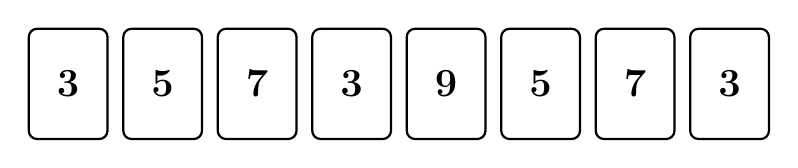
\begin{tikzpicture}
  \foreach \i/\lab in {0/3, 1/5, 2/7, 3/3, 4/9, 5/5, 6/7, 7/3} {
    \draw[thick,rounded corners=3pt] (\i*1.2,0) rectangle ++(1,1.4);
    \node[font=\Large\bfseries] at (\i*1.2+0.5,0.7) {\lab};
  }
\end{tikzpicture}
\end{center}

If one card is drawn at random, what is the probability of drawing a card with the number $3$? Express your answer as a simplified fraction.
\end{questionText}
\correctAnswer{$\frac{3}{8}$}
\explanation{There are $3$ cards labeled $3$ out of $8$ total cards. The probability is $\frac{3}{8}$.}
\end{practiceQuestion}

\begin{practiceQuestion}{9-2-q27}{gsa}
\begin{questionText}
A shelf has the following books:

\begin{center}
\begin{tabular}{|l|c|}
\hline
\textbf{Genre} & \textbf{Number of Books} \\
\hline
Mystery & $9$ \\
\hline
Science Fiction & $6$ \\
\hline
Fantasy & $3$ \\
\hline
Biography & $2$ \\
\hline
\end{tabular}
\end{center}

If a book is chosen at random, what is the probability that it is a mystery or fantasy book? Express your answer as a simplified fraction.
\end{questionText}
\correctAnswer{$\frac{3}{5}$}
\explanation{There are $9 + 3 = 12$ mystery or fantasy books out of $9 + 6 + 3 + 2 = 20$ total. The probability is $\frac{12}{20} = \frac{3}{5}$.}
\end{practiceQuestion}
